%% Physical Review Letters / arXiv style — revtex4-2
\documentclass[aps,pra,twocolumn,superscriptaddress,longbibliography,floatfix]{revtex4-2}

\usepackage{amsmath,amssymb,amsthm}
\newtheorem{theorem}{Theorem}[section]
\newtheorem{lemma}[theorem]{Lemma}
\newtheorem{proposition}[theorem]{Proposition}
\usepackage{graphicx}
\usepackage{xcolor}
\usepackage{booktabs}
\usepackage{hyperref}
\usepackage{bm}
\usepackage{array}
\usepackage{tikz}
\usetikzlibrary{shapes.geometric,positioning,calc,arrows.meta}
\usepackage[caption=false]{subfig}

\hypersetup{colorlinks=true, linkcolor=blue, citecolor=blue, urlcolor=blue}

\newcommand{\vt}{\vartheta}
\newcommand{\al}{\alpha}
\newcommand{\De}{\Delta}
\newcommand{\Tr}{\operatorname{Tr}}
\newcommand{\lmax}{\lambda_{\max}}
\newcommand{\lmin}{\lambda_{\min}}
\newcommand{\QC}{\ensuremath{\text{Quad-}C_5}}

% TikZ styles for graph figures
\tikzset{
  hub/.style  = {circle, draw=black, fill=black!75, text=white,
                 font=\footnotesize\bfseries, inner sep=1.8pt, minimum size=18pt},
  leaf/.style = {circle, draw=black, fill=black!30, text=white,
                 font=\footnotesize\bfseries, inner sep=1.8pt, minimum size=18pt},
  gedge/.style= {thick},
  diagedge/.style = {thick, dashed},
}

\begin{document}

\title{The Quad-$C_5$ Graph: Maximum Contextuality Gap on Eight Vertices}

\author{Ugur Tamer}
\email{utamer24@ku.edu.tr}
\affiliation{Department of Physics, Ko\c{c} University, 34450 Sar{\i}yer, Istanbul, T\"{u}rkiye}

\author{\"{O}zg\"{u}r E.\ M\"{u}stecapl\i{}o\u{g}lu}
\email{omustecap@ku.edu.tr}
\affiliation{Department of Physics, Ko\c{c} University, 34450 Sar{\i}yer, Istanbul, T\"{u}rkiye}
\affiliation{T\"{U}B\.{I}TAK Research Institute for Fundamental Sciences (TBEA), 41470 Gebze, T\"{u}rkiye}

\author{Alper Dizdar}
\email{dizdar@istanbul.edu.tr}
\affiliation{Department of Physics, Faculty of Science,
University of Istanbul, 34134 Vezneciler, Istanbul, T\"{u}rkiye}

\author{Zafer Gedik}
\email{zafer.gedik@sabanciuniv.edu}
\affiliation{Faculty of Engineering and Natural Sciences,
Sabanc{\i} University, Tuzla, Istanbul 34956, T\"{u}rkiye}

\date{\today}

\begin{abstract}
Quantum contextuality rules out classical descriptions in which measurement
outcomes are independent of the compatible measurements performed alongside
them. While the KCBS pentagon provides the minimal qutrit test, identifying
larger but still compact contextuality witnesses remains important for
understanding how contextuality can be organized, amplified, and benchmarked.
We solve the eight-event version of this problem within the graph-theoretic
framework for contextuality. An exhaustive search over all 11{,}117 connected
non-isomorphic graphs with eight vertices identifies a sparse ten-edge graph,
which we call \QC, as the maximum-gap witness. The graph has a larger
absolute contextuality gap than the Wagner graph, a standard eight-vertex
benchmark, despite having fewer exclusivity relations. Its structure is transparent: it is formed from four
overlapping KCBS pentagons, with each edge shared by two pentagons.
We prove that \QC\ is already contextual for a single qutrit by giving
an explicit three-dimensional construction. In this qutrit realization its
contextuality margin equals that of KCBS, whereas its full quantum advantage is
reached numerically in four dimensions and exceeds that of the Wagner graph.
\QC\ therefore provides a compact bridge between minimal qutrit contextuality
and stronger four-dimensional contextuality witnesses.
\end{abstract}

\maketitle

% ─────────────────────────────────────────────────────────────────────────────
\section{Introduction}
% ─────────────────────────────────────────────────────────────────────────────

Quantum contextuality~\cite{KochenSpecker1967} captures an irreducible
tension between quantum mechanics and classical realism: measurement outcomes
cannot, in general, be assigned pre-existing values independently of which
compatible measurements are performed alongside them.
Unlike Bell nonlocality, contextuality does not require spatially separated
subsystems and can already appear in a single finite-dimensional quantum
system. This makes it both a foundational signature of nonclassicality and a
resource for quantum information processing, with established connections to
quantum computation, communication, and
sensing~\cite{Budroni2022,Howard2014,Raussendorf2013}.

Identifying simple yet strong contextuality witnesses is a central goal in
this program. The Klyachko--Can--Binicioğlu--Shumovsky (KCBS) construction
demonstrated that five cyclically compatible measurements on a single spin-1
system are sufficient for a state-dependent contextuality
test~\cite{Klyachko2002,Klyachko2008}. This pentagonal structure became the canonical
minimal qutrit example and was subsequently embedded in the broader family
of $n$-cycle contextuality scenarios, where noncontextual inequalities and
their quantum violations admit analytic characterization~\cite{Araujo2013}.
Such closed-form results are rare: separating classical, quantum, and more
general probabilistic correlations is, in general, a hard problem.

Most experimental contextuality tests have focused on minimal or highly
structured scenarios, such as the KCBS pentagon for qutrits and $n$-cycle
inequalities~\cite{Araujo2013}.
These examples are essential as foundational tests, but recent
resource-theoretic developments motivate a broader question: how can
contextuality be organized, amplified, and benchmarked in larger but still
experimentally manageable exclusivity structures?
This question is especially relevant because contextuality has been connected
to advantages in quantum computation~\cite{Howard2014,Raussendorf2013},
communication~\cite{Gupta2023}, and metrology~\cite{Lostaglio2020}.
From this viewpoint, small-graph optimization plays a role analogous to the
search for compact Bell inequalities or small quantum error-correcting codes:
one seeks the strongest nonclassical signature under limited resources.
Here we address the eight-vertex absolute-gap optimization problem beyond
the analytically understood cycle family and the standard Wagner
benchmark.

A systematic approach to this optimization is provided by the graph-theoretic
framework of Cabello, Severini, and Winter~\cite{Cabello2014}. Each
measurement event is represented as a vertex, and mutually exclusive events
are connected by edges, yielding an exclusivity graph $G=(V,E)$. For
projective measurements, the total event probability satisfies
\begin{equation}
  \al(G) \leq \sum_{i\in V}p_i \leq \vt(G),
  \label{eq:csw_intro}
\end{equation}
where $\al(G)$ is the independence number, giving the noncontextual bound,
and $\vt(G)$ is the Lov\'{a}sz theta number~\cite{Lovasz1979}, giving the
projective quantum bound~\cite{Cabello2014}. The contextuality gap
\begin{equation}
  \De(G) = \vt(G) - \al(G)
  \label{eq:gap_intro}
\end{equation}
measures the separation between quantum and noncontextual descriptions within
this graph model; a larger gap provides a stronger contextuality
resource~\cite{Budroni2022}.

Maximizing the contextuality gap for a fixed vertex count is a nontrivial
combinatorial problem. Adding edges introduces additional exclusivity
constraints that can suppress the quantum value, yet may also lower the
classical bound and reorganize the geometry of the witness.
Consequently, the densest or most symmetric graph need not yield the
strongest contextuality, and even the eight-vertex case presents a
non-obvious optimization landscape.

Known examples chart the structure of this hierarchy. The pentagon $C_5$
realizes the KCBS witness, and the seven-cycle $C_7$ belongs to the
analytically characterized $n$-cycle family~\cite{Araujo2013}. At eight
vertices, the Wagner graph has served as a standard non-cycle
benchmark~\cite{Cabello2014,Lovasz1979}. The full eight-vertex landscape,
however, extends well beyond these symmetric examples, and it is not a priori
clear whether any of these known graphs achieves the global maximum gap or
whether a different, less symmetric structure outperforms them all.

A closely related graph-enumeration program was used in the study of fully
contextual correlations, where the independence number, Lov\'{a}sz theta
number, and fractional packing number were computed for nonisomorphic graphs
with fewer than $11$ vertices~\cite{Amselem2012}. This database was later
used to identify experimentally accessible graphs maximizing the ratio
$\vt(G)/\al(G)$, a relative measure of contextuality
strength~\cite{Canas2016}.
The ratio $\vt(G)/\al(G)$ has since been studied as a graph-based
dimension witness~\cite{Ray2021}, and the CSW exclusivity-graph
framework has been extended to linear games and Bell
inequalities~\cite{Gnacinski2016}.
Building on this graph-theoretic viewpoint, we
focus on a complementary optimization criterion: the absolute CSW gap
$\De(G)=\vt(G)-\al(G)$. This criterion selects compact witnesses with the
largest absolute quantum advantage, determined by the largest additive
separation between the quantum and noncontextual bounds. We use it to
identify the optimal connected eight-vertex graph and then analyze the
structure, dimension dependence, and noise robustness of the resulting
witness. Maximizing $\vt(G)/\al(G)$ favors large relative violations, often
with smaller classical bounds, whereas maximizing $\vt(G)-\al(G)$ favors
large additive separations between the quantum and noncontextual limits.
These two objectives need not select the same graph, and at eight vertices
they do not.

We resolve this question by an exhaustive semidefinite-programming search
over all connected eight-vertex graphs. The numerically certified global maximum is attained by a
ten-edge graph, which we call \QC, that outperforms both the Wagner graph
and every cycle in this vertex range. Its structure is transparent: four
overlapping KCBS pentagons share edges in a regular pattern, providing a
compact mechanism by which KCBS-type contextuality is efficiently combined
within a larger exclusivity graph.

We additionally determine the minimal Hilbert-space dimension needed to
realize this advantage. An explicit three-dimensional orthogonal
representation establishes that \QC\ is already qutrit-contextual, and
numerical evidence shows that its full graph-theoretic quantum value is
first reached in four dimensions. The graph thus bridges minimal qutrit
contextuality and the regime of stronger four-dimensional witnesses;
we compare its noise robustness against both KCBS and Wagner.

The paper is organized as follows. Section~II reviews the graph-theoretic
background and the dimension-restricted quantum quantities used in the
analysis. Section~III describes the exhaustive graph search and numerical
certification. Section~IV presents the \QC\ graph and its structural
properties. Section~V analyzes dimension dependence, noise robustness, and
comparisons with KCBS and Wagner. Section~VI discusses experimental
implementation strategies and platform requirements. Section~VII summarizes
the conclusions. Appendix~A provides the explicit qutrit construction
establishing the analytic lower bound. Appendix~B collects supplementary
tables including the full edge lists, orthogonal representations, and
numerical certification data.

% ─────────────────────────────────────────────────────────────────────────────
\section{Mathematical Background}
% ─────────────────────────────────────────────────────────────────────────────

\subsection{Lov\'{a}sz Theta and Semidefinite Programming}

For a graph $G$ on $n$ vertices with edge set $E$, the Lov\'{a}sz theta
function is given by the semidefinite program~\cite{Lovasz1979,Knuth1994}
\begin{equation}
  \vt(G) = \max_{\substack{X\succeq 0,\;\Tr(X)=1\\
            X_{ij}=0\;\forall(i,j)\in E}}\;
            \mathbf{1}^\top X\,\mathbf{1},
  \label{eq:sdp}
\end{equation}
over the cone of $n\times n$ positive semidefinite matrices.
Equivalently, via the orthonormal representation~\cite{Lovasz1979},
\begin{equation}
  \vt(G) = \max_{|\psi\rangle,\{|v_i\rangle\}}
           \sum_{i=1}^n |\langle\psi|v_i\rangle|^2,
  \label{eq:orth_rep}
\end{equation}
where $\{|v_i\rangle\}\subset\mathbb{C}^d$ are unit vectors with
$\langle v_i|v_j\rangle=0$ for $(i,j)\in E$, and $|\psi\rangle$ is a
handle state.
The Lov\'{a}sz sandwich theorem~\cite{Lovasz1979} gives
$\al(G)\leq\vt(G)\leq\chi(\bar{G})$.
The relaxation over real vectors is tight: $\vt(G)$ equals the maximum
in Eq.~\eqref{eq:orth_rep} even when restricted to $|v_i\rangle\in\mathbb{R}^d$.

\subsection{Quantum Dimension Hierarchy}

The maximum quantum advantage achievable in Hilbert-space dimension $d$
with real orthonormal representations is
\begin{equation}
  \eta_d(G) = \max_{\substack{\{|v_i\rangle\}\subset\mathbb{R}^d,\;
              \|v_i\|=1,\\\langle v_i|v_j\rangle=0\;\forall(i,j)\in E}}
  \lmax\!\!\left(\sum_{i=1}^n |v_i\rangle\!\langle v_i|\right),
  \label{eq:eta_d}
\end{equation}
with $\eta_d(G)\nearrow\vt(G)$ as $d\to n$.
The minimum dimension $d^*$ is
\begin{equation}
  d^*(G) = \min\{d : \eta_d(G)>\al(G)\}.
\end{equation}
Throughout this paper we restrict to rank-one projectors as in the
standard CSW formulation; contextuality witnesses using projectors of
nonunit rank have been studied in Ref.~\cite{Xu2021}.

We distinguish two witness types:
\begin{itemize}
  \item \textbf{Qutrit witness} (here: $d^*=3$, i.e., a graph for which
        $\eta_3(G)>\al(G)$): A single three-level system suffices.
        Note this usage is broader than ``state-independent contextuality
        for spin-1 systems''; we mean only that $d^*=3$.
  \item \textbf{(Numerically indicated) pure two-qubit witness}:
        $\eta_3(G)=\al(G)$ under exhaustive numerical search, and
        $\eta_4(G)>\al(G)$, indicating $d^*=4$.
        Because $\eta_d$ optimization is non-convex, the upper bound
        $\eta_3\leq\al$ for specific graphs carries the caveat discussed
        in the Dimension Classification subsection.
\end{itemize}

% ─────────────────────────────────────────────────────────────────────────────
\section{Methods}
% ─────────────────────────────────────────────────────────────────────────────

\subsection{Exhaustive Graph Enumeration}

McKay's database~\cite{McKay2014} (\texttt{graph8.g6}) contains all
12{,}346 non-isomorphic simple graphs on $n=8$ vertices;
of these, 11{,}117 are connected (OEIS A001349).
We retrieved all graphs, filtered for connectivity, and applied the
analysis pipeline to the connected subset.
Non-isomorphic graphs on $n=5$ and $n=7$ were obtained from NetworkX's
Graph Atlas~\cite{Hagberg2008}.

Although related graph databases exist in the
literature~\cite{Amselem2012,Canas2016,McKay2014}, we performed an
independent enumeration and SDP calculation in order to optimize
$\De(G)=\vt(G)-\al(G)$, verify the ranking, and obtain primal--dual
numerical certificates for the leading graphs.

\subsection{Independence Number}

For each graph $G$ we compute $\al(G)=\omega(\bar{G})$ via maximum-weight
clique search on the complement, implemented in NetworkX.
For $n\leq8$ this is exact; we cross-validated all 11{,}117 results by
independent brute-force enumeration of all $2^8=256$ vertex subsets,
finding perfect agreement across every graph.

\subsection{Lov\'{a}sz Theta via SDP}
\label{sec:method_sdp}

We solve Eq.~\eqref{eq:sdp} using CVXPY~\cite{Diamond2016} with the
SCS solver~\cite{ODonoghue2016} for bulk screening of all 11{,}117
connected graphs; SCS provides typical precision of $10^{-4}$--$10^{-6}$,
sufficient for ranking.
The top 50 candidates were re-solved with the CLARABEL solver
(precision $\sim\!10^{-10}$--$10^{-12}$), whose values are reported
in all tables.
For every graph in the top 50, the SCS--CLARABEL discrepancy is
$|\vt_\text{SCS}-\vt_\text{CLARABEL}|<10^{-7}$ and the CLARABEL primal
feasibility residual satisfies $r_p<4\times10^{-10}$, providing
numerical evidence against artefacts.
The bulk scan completed in under four minutes on a standard laptop CPU.

To test the robustness of the ranking, we recomputed the leading candidates
with two independent conic solvers and repeated the high-accuracy calculations
five times. The resulting numerical ranges for the top three graphs are well
separated: the lower endpoint for \QC\ exceeds the upper endpoint for the
second-ranked graph by $2.94\times10^{-2}$ (Table~\ref{tab:top3cert}; see also Table~\ref{tab:intervals} in Appendix~\ref{app:tables}), many orders of magnitude larger than the reported
primal and dual residuals. We therefore regard the ordering of the leading
graphs, and in particular the uniqueness of \QC\ as the eight-vertex maximizer,
as numerically certified at the reported precision. A fully formal certificate
would require exact arithmetic or independently verifiable interval
primal--dual SDP certificates.

\begin{table*}[tp]
  \caption{Primal--dual certification for the top-3 connected $n=8$
           graphs (CLARABEL solver).
           $\vt_\text{CL}$: primal objective value;
           $r_p = |\mathrm{Tr}\,X-1|$: trace-constraint residual;
           $r_\text{edge} = \max_{(i,j)\in E}|X_{ij}|$: maximum
           edge-constraint violation;
           $\lmin(X)$: smallest eigenvalue of the primal matrix;
           $r_d = y - \vt_\text{CL}$: primal--dual objective gap;
           $\lmin(S)$: smallest eigenvalue of the dual slack matrix.
           Full top-20 data in Appendix~\ref{app:tables}.}
  \label{tab:top3cert}
  \begin{ruledtabular}
  \begin{tabular}{clrccccc}
    Rank & Note &
    $\vt_\text{CL}$ &
    \multicolumn{1}{c}{$r_p$} &
    \multicolumn{1}{c}{$r_\text{edge}$} &
    \multicolumn{1}{c}{$\lmin(X)$} &
    \multicolumn{1}{c}{$r_d$} &
    \multicolumn{1}{c}{$\lmin(S)$} \\
    \hline
     1 & \QC\        & 3.46784 & $+3.7\!\times\!10^{-17}$ & $+3.7\!\times\!10^{-17}$ & $-5.6\!\times\!10^{-9}$ & $-8.5\!\times\!10^{-9}$ & $-2.5\!\times\!10^{-8}$ \\
     2 &            & 3.43845 & $+1.2\!\times\!10^{-19}$ & $+1.2\!\times\!10^{-19}$ & $-1.3\!\times\!10^{-9}$ & $-1.2\!\times\!10^{-9}$ & $-6.8\!\times\!10^{-9}$ \\
     3 & Wagner $W$ & 3.41421 & $+2.1\!\times\!10^{-19}$ & $+2.1\!\times\!10^{-19}$ & $-5.7\!\times\!10^{-9}$ & $+2.5\!\times\!10^{-9}$ & $-1.2\!\times\!10^{-8}$ \\
  \end{tabular}
  \end{ruledtabular}
\end{table*}

\subsection{Dimension Classification via Constrained Optimization}
\label{sec:method_dim}

Computing $\eta_d(G)$ is a non-convex optimization problem that yields a
\emph{lower bound} on $\eta_d$.
We use a three-phase strategy with $N=300$ random restarts:
\begin{enumerate}
  \item \emph{Phase~1} (L-BFGS-B): minimize orthogonality violations
        $\mathcal{L}_1 = \sum_{(i,j)\in E}\langle\hat{v}_i|\hat{v}_j\rangle^2$.
  \item \emph{Phase~2} (L-BFGS-B, penalty method): maximize
        $\lmax\!\bigl(\sum_i|v_i\rangle\!\langle v_i|\bigr)$ with penalty
        weights $w_\perp=50{,}000$, $w_\lambda=0.3$, $w_\mathrm{norm}=5{,}000$.
  \item \emph{Phase~3} (SLSQP): refine with exact equality constraints.
\end{enumerate}
The best $\lmax$ over all restarts is a lower bound on $\eta_d$.
For graphs where all 300 restarts converge to $\lmax=\al$ (the classical
bound), we report $\eta_d\leq\al$ as \emph{numerically indicated}; a
formal upper-bound certificate would require an SDP relaxation over
$d$-dimensional representations, which is left for future work.

\subsection{Closed-Form Identification via PSLQ}

To identify algebraic closed forms, we apply the PSLQ
algorithm~\cite{Bailey1999} at 50-decimal-digit precision
(\texttt{mpmath} library).
We validate each candidate polynomial $P$ of degree $k$ via the residual
test: the ratio
\begin{equation}
  r = |P(x)|/\bigl(|P'(x)|\cdot\varepsilon_{\rm SDP}\bigr)
\end{equation}
must satisfy $r\ll 1$ for the relation to be genuine rather than a
numerical coincidence ($\varepsilon_{\rm SDP}\approx10^{-15}$ is the
CLARABEL precision).
We search for integer relations of degree $k\leq4$ with coefficient bound
$|c_i|\leq10^6$; the unique solution at $k=2$ is $x^2-2x-4=0$.
PSLQ detection is not a formal algebraic proof but constitutes high-confidence
numerical identification~\cite{Bailey1999}; a formal proof would require
an independent algebraic construction or exact-arithmetic SDP.

% ─────────────────────────────────────────────────────────────────────────────
\section{Results}
\label{sec:results}
% ─────────────────────────────────────────────────────────────────────────────

\subsection{Reference Results: $n=5$ and $n=7$}

For $n=5$, the maximum contextuality gap is achieved by the five-cycle $C_5$
(the KCBS exclusion graph~\cite{Klyachko2008}):
\begin{equation}
  \al(C_5)=2,\quad\vt(C_5)=\sqrt{5},\quad\De(C_5)=\sqrt{5}-2\approx0.236.
\end{equation}
For $n=7$, the maximum is the seven-cycle $C_7$~\cite{Araujo2013}, which
we verify by exhaustive SDP search over all 853 connected non-isomorphic
$n=7$ graphs using the same pipeline:
\begin{equation}
  \vt(C_7)=\frac{7\cos(\pi/7)}{1+\cos(\pi/7)}\approx3.318,\quad
  \De(C_7)\approx0.318.
\end{equation}
Both $C_5$ and $C_7$ are qutrit witnesses ($d^*=3$).

\subsection{Exhaustive Search over $n=8$}

Table~\ref{tab:n8_top10} lists the top-10 graphs by $\De$ from the
exhaustive search.
\QC\ achieves $\De=0.46784$, exceeding the Wagner graph $W$
(Rank~3) by $0.46784-0.41421=0.05363$, while using only 10 edges compared
to $W$'s 12.

\begin{table}[tp]
  \caption{Top-10 connected graphs on $n=8$ vertices by contextuality gap
           $\De=\vt-\al$ (CLARABEL values), from exhaustive search over the
           11{,}117 connected non-isomorphic simple 8-vertex graphs.
           The column $\vt/\al$ is the relative contextuality measure
           used in earlier graph searches~\cite{Canas2016,Ray2021}; its $n{=}8$
           maximizer (Rank~7, $\dagger$, the CHSH-type graph discussed
           in Ref.~\cite{Canas2016})
           differs from the gap maximizer (\QC, Rank~1).}
  \label{tab:n8_top10}
  \begin{ruledtabular}
  \begin{tabular}{clrrrrrr}
    Rank & Note & \multicolumn{1}{c}{$|E|$} &
          \multicolumn{1}{c}{$\al$} &
          \multicolumn{1}{c}{$\vt$} &
          \multicolumn{1}{c}{$\De$} &
          \multicolumn{1}{c}{$\vt/\al$} \\
    \hline
    1  & \QC\ ($n{=}8$ gap max)        & 10 & 3 & 3.46784 & 0.46784 & 1.15595 \\
    2  &                              & 11 & 3 & 3.43845 & 0.43845 & 1.14615 \\
    3  & Wagner $W$                   & 12 & 3 & 3.41421 & 0.41421 & 1.13807 \\
    4  &                              & 11 & 3 & 3.37228 & 0.37228 & 1.12409 \\
    5  &                              & 12 & 3 & 3.37228 & 0.37228 & 1.12409 \\
    6  &                              & 10 & 3 & 3.37228 & 0.37228 & 1.12409 \\
    7  & $\dagger$ CHSH-type graph     & 16 & 2 & 2.34315 & 0.34315 & 1.17157 \\
    8  &                              & 11 & 3 & 3.33804 & 0.33804 & 1.11268 \\
    9  &                              & 17 & 2 & 2.33804 & 0.33804 & 1.16902 \\
    10 &                              & 18 & 2 & 2.33333 & 0.33333 & 1.16667 \\
  \end{tabular}
  \end{ruledtabular}
\end{table}

\subsection{Structure of the \QC\ Graph}

The graph6 canonical encoding~\cite{McKay2014} of this graph is
\verb|GCQb`o|, which we retain as a reproducibility identifier.
\QC\ has vertex set $V=\{0,1,\ldots,7\}$ and edge set
\begin{align}
  E = \{&(0,3),(0,5),(1,4),(1,6),(2,5),(2,6),\nonumber\\
         &(2,7),(3,6),(3,7),(4,7)\}.
  \label{eq:qc_edges}
\end{align}
Its degree sequence is $(2,2,2,2,3,3,3,3)$: vertices $\{0,1,4,5\}$ have
degree~2 (``leaf'' nodes) and vertices $\{2,3,6,7\}$ have degree~3
(``hub'' nodes).
The graph is neither regular nor vertex-transitive.
The four hub nodes $\{2,3,6,7\}$ form a complete bipartite subgraph
$K_{2,2}$ (bipartition $\{2,3\}\times\{6,7\}$), while the leaf nodes
attach as two pendant paths $3{-}0{-}5{-}2$ and $6{-}1{-}4{-}7$,
each bridging one hub pair through two degree-2 vertices.

Figure~\ref{fig:graphs} visualizes \QC\ alongside the Wagner
graph $W$ for comparison.

\begin{figure}[tp]
\centering
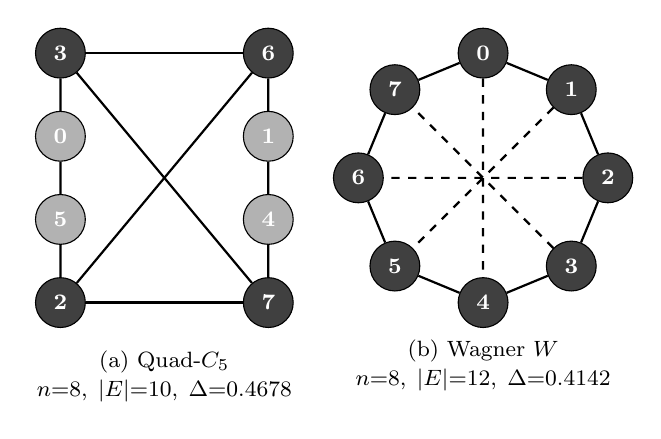
\begin{tikzpicture}[scale=0.88]

%── (a) Quad-C5: symmetric two-column layout ──────────────────────
\begin{scope}[xshift=-2.2cm]
  % Left column: hub(3)–leaf(0)–leaf(5)–hub(2)
  \node[hub]  (v3) at (-1.5,  1.8) {3};
  \node[leaf] (v0) at (-1.5,  0.6) {0};
  \node[leaf] (v5) at (-1.5, -0.6) {5};
  \node[hub]  (v2) at (-1.5, -1.8) {2};
  % Right column: hub(6)–leaf(1)–leaf(4)–hub(7)
  \node[hub]  (v6) at ( 1.5,  1.8) {6};
  \node[leaf] (v1) at ( 1.5,  0.6) {1};
  \node[leaf] (v4) at ( 1.5, -0.6) {4};
  \node[hub]  (v7) at ( 1.5, -1.8) {7};
  % Left pendant path: 3–0–5–2
  \draw[gedge] (v3)--(v0)--(v5)--(v2);
  % Right pendant path: 6–1–4–7
  \draw[gedge] (v6)--(v1)--(v4)--(v7);
  % K_{2,2} core: horizontal edges
  \draw[gedge] (v3)--(v6);
  \draw[gedge] (v2)--(v7);
  % K_{2,2} core: diagonal edges
  \draw[gedge] (v3)--(v7);
  \draw[gedge] (v2)--(v6);
  \node[below=5pt, align=center, font=\footnotesize] at (0,-2.15)
    {(a)~\QC\\[1pt]
     $n{=}8,\;|E|{=}10,\;\De{=}0.4678$};
\end{scope}

%── (b) Wagner W: standard circular layout ───────────────────────
\begin{scope}[xshift=2.4cm]
  \def\R{1.8}
  \foreach \k/\ang in {0/90,1/45,2/0,3/315,4/270,5/225,6/180,7/135}{
    \node[hub] (w\k) at (\ang:\R) {\k};
  }
  \draw[gedge] (w0)--(w1)--(w2)--(w3)--(w4)--(w5)--(w6)--(w7)--(w0);
  \draw[diagedge] (w0)--(w4) (w1)--(w5) (w2)--(w6) (w3)--(w7);
  \node[below=5pt, align=center, font=\footnotesize] at (0,-\R-0.2)
    {(b)~Wagner $W$\\[1pt]
     $n{=}8,\;|E|{=}12,\;\De{=}0.4142$};
\end{scope}

\end{tikzpicture}
\caption{%
  (a)~The optimal witness \QC\ ($\De=0.4678$, 10~edges).
  Dark (hub) nodes have degree~3; light (leaf) nodes have degree~2.
  The four hub nodes $\{2,3,6,7\}$ form a $K_{2,2}$ core;
  leaves attach via two pendant paths $3{-}0{-}5{-}2$ (left column)
  and $6{-}1{-}4{-}7$ (right column).
  (b)~The Wagner graph $W$ ($\De=0.4142$, 12~edges, 3-regular);
  dashed lines are the four ``long diagonals'' of the $C_8$ cycle.
  \QC\ surpasses $W$ by $13\%$ in contextuality gap with
  two fewer edges.}
\label{fig:graphs}
\end{figure}

A defining structural feature is that \QC\ contains exactly four
induced five-cycles (KCBS pentagons), listed in Table~\ref{tab:c5_subgraphs}.
Crucially, \emph{every} one of the 10 edges belongs to exactly two of the
four $C_5$ subgraphs---a perfect two-fold edge coverage.

The adjacency spectrum of \QC\ is displayed in
Table~\ref{tab:spectrum} in Appendix~\ref{app:tables}.
Six of the eight eigenvalues belong to the golden-ratio field
$\mathbb{Q}(\sqrt{5})$: $\{1+\varphi,\; \varphi^{-1}(\times 2),\;
1-\varphi^{-1},\; -\varphi(\times 2)\}$, where $\varphi=(1+\sqrt{5})/2$.
This is a direct spectral fingerprint of the embedded $C_5$ subgraphs.
The remaining two eigenvalues ($\approx\!+1.303$ and $\approx\!-2.303$)
do not lie in $\mathbb{Q}(\sqrt{5})$; their structural origin within
the graph is an open question.

\subsection{Edge Lists for the Top-6 Graphs}

Complete edge lists for reproducibility are given in
Table~\ref{tab:edgelists} in Appendix~\ref{app:tables}.

\subsection{Dimension Classification}
\label{sec:dim_class}

Table~\ref{tab:dim_class} in Appendix~\ref{app:tables} presents $\eta_3$ and dimension classifications.
Ranks~1, 2, 4, and~6 are confirmed qutrit witnesses: the 300-restart
optimization finds configurations with $\lmax>3$, providing a constructive
lower bound $\eta_3>\al$.
The Wagner graph (Rank~3) and Rank~5 return $\lmax=3.000$ across all 300
restarts, consistent with $\eta_3=\al=3$ (numerically indicated pure
two-qubit witnesses).

We note that the claim $\eta_3(W)=\al=3$ is a \emph{lower-bound} result:
the optimization confirms that the best 3D representation found attains
$\lmax=\al$, but without an SDP upper-bound verification one cannot rule out
a 3D configuration with $\lmax>3$ that the heuristic failed to find.
For the Wagner graph, the high regularity and well-studied symmetry
($\text{Aut}(W)\cong D_4\times\mathbb{Z}_2$, order 16) make the numerical
finding credible, and a formal $d^*=4$ proof remains an open question.

The numerically indicated $\eta_3$ value $1+\sqrt{5}\approx3.236$ appears
for Ranks~1, 2, and~4; its analytic lower bound is established in the
next subsection.

\subsection{Orthogonal Vector Representations}

Table~\ref{tab:orth_reps} in Appendix~\ref{app:tables} summarizes the achieved $\lmax$ values for the
key configurations.
For \QC\ at $d=3$, all 300 restarts converge to $\lmax=3.236068$ with
maximum orthogonality error $<2.3\times10^{-14}$, confirming the qutrit
advantage is robustly attained.
At $d=4$, the optimization converges to $\lmax=3.467844\approx\vt$, with
orthogonality error $<3.3\times10^{-14}$, confirming that the full
Lov\'{a}sz bound is numerically saturated in four dimensions.

\subsection{Analytic qutrit lower bound and numerical evidence for tightness}

The optimized three-dimensional value found in all numerical runs is
\begin{equation}
  \eta_3^{\rm num}(\QC) = 1+\sqrt{5} \approx 3.23607,
  \label{eq:eta3_num}
\end{equation}
identified via PSLQ applied to the numerically obtained $\eta_3\approx3.236068$
at 50-digit precision.
The degree-2 polynomial $P(x)=x^2-2x-4$ has positive root $1+\sqrt{5}$, and
the residual test yields
$r=|P(\eta_3)|/\bigl(|P'(\eta_3)|\cdot\varepsilon_{\rm SDP}\bigr)\approx0.3\ll1$,
confirming a genuine algebraic relation.
We prove the analytic lower bound
\begin{equation}
  \eta_3(\QC) \geq 1+\sqrt{5}
  \label{eq:eta3_lb}
\end{equation}
by constructing an explicit orthogonal representation in $\mathbb{R}^3$
(Appendix~\ref{app:analytic}).
Extensive high-precision optimization and PSLQ recognition indicate that
this bound is tight, although a formal dimension-constrained upper bound
remains open.

A representative set of unit vectors $\{|v_i\rangle\}\subset\mathbb{R}^3$
achieving $\lmax=1+\sqrt{5}$ (orthogonality error $<2.5\times10^{-14}$,
obtained from 500 independent restarts using SLSQP with explicit orthogonality
constraints, all converging to the same $\lmax$ with
$|\lmax-(1+\sqrt{5})|<3\times10^{-13}$)
is given in Table~\ref{tab:unit_vecs}.

This numerically determined value connects \QC\ to the KCBS
pentagon: both $\vt(C_5)=\sqrt{5}$ and $\eta_3(\QC)=1+\sqrt{5}$
lie in $\mathbb{Q}(\sqrt{5})$.
The same $\eta_3$ value also appears for Ranks~2 and~4 (Table~\ref{tab:dim_class} in Appendix~\ref{app:tables}).

By contrast, the candidate polynomial for $\vt(\QC)$
at 15-digit precision has $r\approx20\gg1$ and is a false positive.
A reliable closed form for $\vt$ requires a high-precision solver such as
SDPA-GMP~\cite{Nakata2010} at $\geq30$ significant digits.

\subsection{Known-Graph Hierarchy}

\begin{equation}
  \De(C_5) < \De(C_7) < \De(W) < \De(\QC),
\end{equation}
with numerical values in Table~\ref{tab:hierarchy} in Appendix~\ref{app:tables}.

% ─────────────────────────────────────────────────────────────────────────────
\section{Discussion}
% ─────────────────────────────────────────────────────────────────────────────

\subsection{Efficiency of Contextuality Geometry}

The main surprise is that \QC\ achieves a larger contextuality
gap than $W$ with \emph{two fewer edges}.
Adding an edge to an exclusion graph imposes an additional orthogonality
constraint in Eq.~\eqref{eq:sdp}, generically reducing $\vt(G)$ while
leaving $\al(G)$ unchanged or reducing it.
Naively, fewer edges should correlate with a smaller gap.
The fact that the optimal graph is sparser than the previously leading example points
to a more efficient contextuality geometry: the four interlocking KCBS
pentagons in \QC\ encode more quantum advantage per edge than
the symmetric 3-regular structure of $W$.

The two-fold edge coverage by the four $C_5$ subgraphs
(Table~\ref{tab:c5_subgraphs} in Appendix~\ref{app:tables}) is a candidate structural explanation,
though a formal proof of this connection remains open.
This is related to properties of the Lov\'{a}sz theta under graph
combinations~\cite{Lovasz1979}: shared edges prevent full cancellation
of the individual contributions, allowing the four $C_5$ copies to
reinforce each other.

\subsection{Physical Significance of the Qutrit--Two-Qubit Distinction}

A qutrit witness ($d^*=3$) is testable on a single three-level system:
photon orbital angular momentum~\cite{Molina-Terriza2007}
or an atomic $\Lambda$-system~\cite{Hu2016}.
Such systems avoid the engineering complexity of entangled bipartite
platforms and are more resilient to certain decoherence channels.

A (numerically indicated) pure two-qubit witness ($d^*=4$) cannot exploit
contextuality in any three-dimensional Hilbert-space embedding: the
orthogonality constraints for its edge set require a four-dimensional
space.
This makes such witnesses more demanding experimentally but potentially more
useful as probes of composite-system structure.
Contextuality of this kind remains distinct from Bell nonlocality, as no
entanglement between the two qubits is required~\cite{Spekkens2005,Porto2024}.

Remarkably, $W$ and Rank~5 are non-isomorphic graphs but share identical
numerically indicated dimensional behavior ($\eta_3=\al$, $\eta_4>\al$).
This structural coincidence suggests an underlying algebraic invariant
beyond $\vt$ and $\al$ that governs dimensional rigidity.

\subsection{Noise Robustness under Depolarizing Noise}

We analyze noise robustness via the standard depolarizing channel
$\rho_\text{noisy} = v\,\rho + (1-v)\,I/d$,
where $v\in[0,1]$ is the visibility.
Since each observable is a rank-1 projector with $\mathrm{Tr}(P_i)=1$,
the observable sum under this channel becomes
$S(v) = v\,\eta_d(G) + (1-v)\,n/d$,
and contextuality is certified whenever $S(v)>\al(G)$.
Solving for the minimum visibility required yields the
\emph{critical visibility}
\begin{equation}
  v^* = \frac{\al(G) - n/d}{\eta_d(G) - n/d},
  \label{eq:vstar}
\end{equation}
with noise tolerance $1-v^*$.
Table~\ref{tab:noise} lists the values for the witnesses studied here.

\begin{table}[tp]
  \caption{Critical visibility $v^*$ and noise tolerance $1-v^*$ under
           depolarizing noise, computed from Eq.~\eqref{eq:vstar}.
           The unrestricted Lov\'{a}sz values $\vt$ are obtained from the
           high-accuracy SDP calculations in Table~\ref{tab:intervals} in Appendix~\ref{app:tables}.
           The dimension-constrained $\eta_3$ values are obtained from the
           nonconvex orthogonal-representation optimization described in
           Sec.~\ref{sec:method_dim}.}
  \label{tab:noise}
  \begin{ruledtabular}
  \begin{tabular}{lrrrr cc}
    Graph & $n$ & $\al$ & $\eta_d$ & $d$ & $v^*$ & $1-v^*$ \\
    \hline
    $C_5$ (KCBS)        & 5 & 2 & 2.23607 & 3 & 0.5854 & 0.4146 \\
    $C_7$               & 7 & 3 & 3.31767 & 3 & 0.6773 & 0.3227 \\
    \QC\ ($d=3$)        & 8 & 3 & 3.23607 & 3 & 0.5854 & 0.4146 \\
    \QC\ ($d=4$)        & 8 & 3 & 3.46784 & 4 & 0.6813 & 0.3187 \\
    Wagner $W$ ($d=4$)  & 8 & 3 & 3.41421 & 4 & 0.7071 & 0.2929 \\
  \end{tabular}
  \end{ruledtabular}
\end{table}

The most striking entry in Table~\ref{tab:noise} is the exact coincidence
$v^*(\text{KCBS})=v^*(\QC,d{=}3)$: despite having three more vertices,
\QC\ at $d=3$ tolerates up to $41.5\%$ depolarizing noise---the same
threshold as the simplest known contextuality witness.
Substituting the established values into Eq.~\eqref{eq:vstar},
\begin{align}
  v^*(\text{KCBS}) &= \frac{2-\tfrac{5}{3}}{\sqrt{5}-\tfrac{5}{3}}
                    = \frac{1}{3\sqrt{5}-5}, \label{eq:vstar_kcbs}\\[2pt]
  v^*(\QC,\,d{=}3) &= \frac{3-\tfrac{8}{3}}{(1+\sqrt{5})-\tfrac{8}{3}}
                    = \frac{1}{3\sqrt{5}-5}, \label{eq:vstar_qc}
\end{align}
confirming the equality analytically.
The coincidence is explained by a \emph{uniform shift}: going from $C_5$
to \QC, all three parameters entering Eq.~\eqref{eq:vstar} increase
by the same amount, $\Delta\al=\Delta\eta_3=\Delta(n/d)=1$.
Since the ratio in Eq.~\eqref{eq:vstar} is invariant under any common
additive shift $k$,
\begin{equation}
  \frac{(\al+k)-(n/d+k)}{(\eta+k)-(n/d+k)} = \frac{\al-n/d}{\eta-n/d},
  \label{eq:shift_invariance}
\end{equation}
the critical visibilities are identical.
The shift $\Delta(n/d)=1$ follows immediately: \QC\ has $n=8=5+d$ vertices.
Why $\Delta\al=\Delta\eta_3=1$ hold simultaneously is an open structural question
not resolved by the exhaustive search.

This equality has a direct experimental consequence: any qutrit apparatus
sufficient for a KCBS test can certify \QC\ contextuality without any
relaxation of the noise requirements.
At $d=3$ both witnesses achieve the same quantum advantage $\eta_3-\al=\sqrt{5}-2\approx0.236$;
the larger Lov\'{a}sz gap $\De(\QC)=0.468$ reflects the full
quantum potential of the graph and is accessible at $d=4$.

At $d=4$, \QC\ also strictly outperforms Wagner in noise robustness.
The numerically indicated value $\vt(W)=2+\sqrt{2}$ yields
$v^*(W,d{=}4)=1/\sqrt{2}\approx0.707$,
whereas $v^*(\QC,d{=}4)\approx0.681$, a reduction of $2.6\%$.
Any experiment achieving visibility $v\in[0.681,\,0.707]$ can therefore
certify \QC\ contextuality but not Wagner contextuality.

Finally, the $C_7$ entry in Table~\ref{tab:noise} illustrates that a larger
gap $\De$ does not guarantee better noise robustness.
Despite $\De(C_7)=0.318>\De(\text{KCBS})=0.236$, $C_7$ requires strictly
higher visibility ($v^*=0.677>0.585$).
The reason is structural: the larger vertex count raises the mixed-state
baseline $n/d=7/3$, compressing the gap between the classical bound and
the quantum value and eroding the advantage faster under noise.
The critical visibility $v^*$, not $\De$ alone, is the operationally
correct figure of merit for experimental feasibility.

\subsection{Algebraic Connection to KCBS via $\mathbb{Q}(\sqrt{5})$}

The high-confidence identification $\eta_3(\QC)=1+\sqrt{5}$
reveals a deep algebraic link to the KCBS scenario.
Both $\vt(C_5)=\sqrt{5}$ and $\eta_3(\QC)=1+\sqrt{5}$ lie in
$\mathbb{Q}(\sqrt{5})$.
Equivalently, the three-dimensional advantage of \QC\ above
the classical bound $\al=3$ is exactly $\sqrt{5}$---one unit of KCBS
advantage above the classical floor.

The adjacency spectrum reinforces this picture: the six golden-ratio
eigenvalues $\{1+\varphi,\; \varphi^{-1}(\times 2),\; 1-\varphi^{-1},\;
-\varphi(\times 2)\}$ are the spectral fingerprint of graphs built from
$C_5$ building blocks~\cite{Cvetkovic1980}, providing spectral-graph-theory
evidence that the contextuality advantage is inherited from the KCBS
subgraphs.

% ─────────────────────────────────────────────────────────────────────────────
\section{Experimental Feasibility}
\label{sec:ExperimentalFeasibility}
% ─────────────────────────────────────────────────────────────────────────────

From a fundamental standpoint, KCBS is the simplest qutrit witness, requiring
only five events; this also makes it attractive for experimental tests of
foundational contextuality~\cite{Klyachko2008,Hu2016}.
On the other hand, contextuality can have practical value and hence benefit
from scaling.
The \QC\ graph addresses how contextuality can be organized and enhanced in a
compact eight-event exclusivity structure.

A qutrit implementation requires eight rank-one projectors
\begin{equation}
  \Pi_i = |v_i\rangle\langle v_i|, \qquad i=0,\ldots,7,
\end{equation}
satisfying
\begin{equation}
  \Pi_i\Pi_j = 0 \qquad \text{for every edge }(i,j)\in E.
\end{equation}
The explicit construction in Appendix~\ref{app:analytic} provides such a
representation and therefore gives a direct experimental prescription.
The optimal input state is the eigenstate of
\begin{equation}
  M = \sum_i \Pi_i
\end{equation}
with largest eigenvalue. In the qutrit construction this state yields
\begin{equation}
  \sum_i \langle\Pi_i\rangle = 1+\sqrt{5}
\end{equation}
(see Eq.~\eqref{eq:psi_star} in Appendix~\ref{app:analytic}).

The qutrit realization is non-injective: two pairs of nonadjacent vertices
are represented by identical projectors ($v_0=v_6$ and $v_2=v_3$).
Operationally, this corresponds to repeated projector terms appearing in
different exclusivity contexts.
This is consistent with the graph-theoretic orthogonal-representation
framework, but it also shows why the qutrit advantage remains KCBS-like.
The larger contextuality gap of \QC\ is obtained only in a four-dimensional
realization, where the full Lov\'{a}sz value is reached numerically.

Possible platforms include spin-1 ion-trap and solid-state
systems~\cite{Klyachko2008,Kirchmair2009,Jerger2016}, photonic path or
orbital-angular-momentum
qutrits~\cite{Molina-Terriza2007,Hu2016,Lapkiewicz2011},
NMR qutrits~\cite{Budroni2022,Dogra2015}, and four-level photonic or
two-qubit systems~\cite{Amselem2009}.
In a four-dimensional implementation, \QC\ becomes experimentally more
appealing than the Wagner benchmark because it requires a strictly lower
critical visibility under depolarizing noise ($v^*\approx0.681$
vs.\ $v^*(W)\approx0.707$).

% ─────────────────────────────────────────────────────────────────────────────
\section{Conclusion}
% ─────────────────────────────────────────────────────────────────────────────

We have carried out an exhaustive search over all 11{,}117 connected
non-isomorphic simple graphs on eight vertices and identified
\QC---an 8-vertex, 10-edge graph containing four interlocking
KCBS pentagons---as the numerically certified unique maximizer of the contextuality gap for $n=8$.
With $\De=0.46784$, it surpasses the Wagner graph ($\De\approx0.414$) by
$\sim\!13\%$ while using two fewer edges.

Unlike the Wagner graph, which numerical evidence indicates requires a
four-dimensional Hilbert space, \QC\ is a confirmed qutrit
witness: high-precision numerics indicate that
$\eta_3(\QC)=1+\sqrt{5}$, placing this value in the same
algebraic field $\mathbb{Q}(\sqrt{5})$ as the KCBS pentagon.
In four dimensions, the full Lov\'{a}sz bound is saturated with
orthogonality error below $10^{-13}$.

A depolarizing noise analysis reveals that \QC\ at $d=3$ shares the
critical visibility $v^*=1/(3\sqrt{5}-5)\approx0.585$ of the KCBS witness,
an equality that follows analytically from a uniform shift of the graph
parameters $\al$, $\eta_3$, and $n/d$.
Any qutrit apparatus sufficient for a KCBS test can therefore certify
\QC\ contextuality without relaxing noise requirements.
At $d=4$, \QC\ also strictly outperforms the Wagner graph in noise
robustness, requiring $2.6\%$ less visibility.

The present optimization is complementary to earlier graph-based searches
for fully contextual correlations~\cite{Amselem2012} and for graphs
maximizing the relative measure $\vt(G)/\al(G)$~\cite{Canas2016}.
Those searches identify different extremal structures. Here the objective
is the absolute CSW gap $\De(G)=\vt(G)-\al(G)$, for which \QC\ is the
eight-vertex maximizer in our exhaustive search.

These results show that the optimal eight-vertex exclusivity graph is already
qutrit-contextual, while its full Lov\'{a}sz value gives a stronger
four-dimensional contextuality benchmark than the Wagner graph.
They provide concrete graph structures suitable for experimental tests in
three-level and four-level quantum systems.
The finding that the $n=8$ maximum requires \emph{fewer} edges than the
Wagner graph suggests that denser exclusion graphs do not always yield
stronger contextuality; the relationship between graph sparsity and
contextuality strength warrants systematic future investigation.

% ─────────────────────────────────────────────────────────────────────────────
\section*{Data Availability}

All graph data derive from the publicly available McKay database
(\texttt{graph8.g6},
\url{https://users.cecs.anu.edu.au/~bdm/data/}).
Complete edge lists are given in Table~\ref{tab:edgelists} (Appendix~\ref{app:tables});
All Python scripts and data files are publicly available at
\url{https://github.com/ugurtamerphys/quad-c5-contextuality} and archived on
Zenodo~\cite{Tamer2026zenodo}.

\begin{acknowledgments}
We thank Ad\'{a}n Cabello for helpful correspondence and for drawing our
attention to earlier graph-database studies of contextuality and their
experimental realizations.
We also thank Sena Nur Tamer, Julie Zeynep Pagy, and Serta\c{c} F{\i}rat
for useful discussions.
Part of this work was carried out at Bilimler K\"{o}y\"{u}.
The numerical calculations used the open-source packages CVXPY, NetworkX,
SCS, CLARABEL, and mpmath.
The authors used artificial-intelligence-assisted language-editing tools to improve grammar,
clarity, and readability of parts of the manuscript.
All scientific ideas, calculations, analysis, interpretation of results,
conclusions, and final text were developed, checked, and approved by the
authors.
\end{acknowledgments}

% ─────────────────────────────────────────────────────────────────────────────
\appendix
% ─────────────────────────────────────────────────────────────────────────────
\section{Analytic Lower Bound: $\eta_3(\QC)\geq 1+\sqrt{5}$}
\label{app:analytic}

We construct an explicit orthogonal representation of $\QC$ in $\mathbb{R}^3$
achieving $\lambda_{\max}=1+\sqrt{5}$, thereby proving $\eta_3(\QC)\geq 1+\sqrt{5}$.

\subsection{Graph Structure}

The \QC\ graph has vertex set $\{0,\ldots,7\}$ and edge set
\begin{align*}
  E = \{&(0,3),(0,5),(1,4),(1,6),(2,5),\\
        &(2,6),(2,7),(3,6),(3,7),(4,7)\}.
\end{align*}
Figure~\ref{fig:qc5_graph} shows the graph together with its four embedded
$C_5$ pentagons.

\begin{figure}[h]
\centering
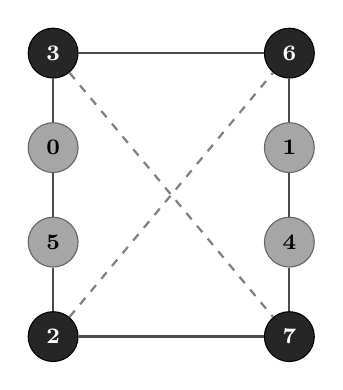
\begin{tikzpicture}[
  hub/.style={circle, fill=black!85, draw=black,
              minimum size=18pt, inner sep=0pt,
              font=\footnotesize\bfseries\color{white}},
  leaf/.style={circle, fill=black!35, draw=black!60,
               minimum size=18pt, inner sep=0pt,
               font=\footnotesize\bfseries},
  gedge/.style={thick, black!70},
  diagedge/.style={thick, black!50, dashed}
]
% Left column: hub(3)--leaf(0)--leaf(5)--hub(2)
\node[hub]  (v3) at (-1.5,  1.8) {3};
\node[leaf] (v0) at (-1.5,  0.6) {0};
\node[leaf] (v5) at (-1.5, -0.6) {5};
\node[hub]  (v2) at (-1.5, -1.8) {2};
% Right column: hub(6)--leaf(1)--leaf(4)--hub(7)
\node[hub]  (v6) at ( 1.5,  1.8) {6};
\node[leaf] (v1) at ( 1.5,  0.6) {1};
\node[leaf] (v4) at ( 1.5, -0.6) {4};
\node[hub]  (v7) at ( 1.5, -1.8) {7};
% Pendant paths
\draw[gedge] (v3)--(v0)--(v5)--(v2);
\draw[gedge] (v6)--(v1)--(v4)--(v7);
% K_{2,2} horizontal edges
\draw[gedge] (v3)--(v6);
\draw[gedge] (v2)--(v7);
% K_{2,2} diagonal edges
\draw[diagedge] (v3)--(v7);
\draw[diagedge] (v2)--(v6);
\end{tikzpicture}
\caption{The \QC\ graph ($n=8$, $m=10$) in the same layout as
         Fig.~\ref{fig:graphs}(a).
         Dark (hub) nodes $\{2,3,6,7\}$ have degree~3;
         light (leaf) nodes $\{0,1,4,5\}$ have degree~2.
         Dashed edges are the two $K_{2,2}$ diagonals $(2,6)$ and $(3,7)$.}
\label{fig:qc5_graph}
\end{figure}

It contains exactly four induced $C_5$ pentagons, shown in
Fig.~\ref{fig:c5_subgraphs}:
$C_5^{(1)}$: $0\text{-}3\text{-}6\text{-}2\text{-}5\text{-}0$;\quad
$C_5^{(2)}$: $0\text{-}3\text{-}7\text{-}2\text{-}5\text{-}0$;\quad
$C_5^{(3)}$: $1\text{-}4\text{-}7\text{-}2\text{-}6\text{-}1$;\quad
$C_5^{(4)}$: $1\text{-}4\text{-}7\text{-}3\text{-}6\text{-}1$.
Every edge of $\QC$ belongs to exactly two of these pentagons.

% Helper macro: draw QC in the same two-column layout as Fig.1(a)
% #1 = highlighted edge commands, #2 = highlighted vertex commands
\newcommand{\drawQCsmall}[2]{%
\begin{tikzpicture}[
  vxB/.style={circle,fill=black!25,draw=black!45,
              minimum size=14pt,inner sep=0pt,
              font=\scriptsize},
  vxH/.style={circle,minimum size=14pt,inner sep=0pt,
              font=\scriptsize\bfseries\color{white}},
  egB/.style={thick,black!25},
  egH/.style={very thick},
  scale=0.62
]
\coordinate (v3) at (-1.5, 1.8);
\coordinate (v0) at (-1.5, 0.6);
\coordinate (v5) at (-1.5,-0.6);
\coordinate (v2) at (-1.5,-1.8);
\coordinate (v6) at ( 1.5, 1.8);
\coordinate (v1) at ( 1.5, 0.6);
\coordinate (v4) at ( 1.5,-0.6);
\coordinate (v7) at ( 1.5,-1.8);
\draw[egB] (v3)--(v0)--(v5)--(v2);
\draw[egB] (v6)--(v1)--(v4)--(v7);
\draw[egB] (v3)--(v6) (v2)--(v7) (v3)--(v7) (v2)--(v6);
#1
\foreach \v in {v0,v1,v2,v3,v4,v5,v6,v7}{\node[vxB] at (\v) {};}
#2
\end{tikzpicture}%
}

\begin{figure*}[!t]
\centering
\subfloat[$C_5^{(1)}$: $3\text{-}0\text{-}5\text{-}2\text{-}6$]{%
\begin{minipage}[b]{0.23\textwidth}\centering
\drawQCsmall{%
  \draw[egH,red!75!black] (v3)--(v0)--(v5)--(v2)--(v6)--(v3);
}{%
  \node[vxH,fill=red!75!black,draw=red!75!black] at (v3) {3};
  \node[vxH,fill=red!75!black,draw=red!75!black] at (v0) {0};
  \node[vxH,fill=red!75!black,draw=red!75!black] at (v5) {5};
  \node[vxH,fill=red!75!black,draw=red!75!black] at (v2) {2};
  \node[vxH,fill=red!75!black,draw=red!75!black] at (v6) {6};
}
\end{minipage}}
\hfill
\subfloat[$C_5^{(2)}$: $3\text{-}0\text{-}5\text{-}2\text{-}7$]{%
\begin{minipage}[b]{0.23\textwidth}\centering
\drawQCsmall{%
  \draw[egH,blue!75!black] (v3)--(v0)--(v5)--(v2)--(v7)--(v3);
}{%
  \node[vxH,fill=blue!75!black,draw=blue!75!black] at (v3) {3};
  \node[vxH,fill=blue!75!black,draw=blue!75!black] at (v0) {0};
  \node[vxH,fill=blue!75!black,draw=blue!75!black] at (v5) {5};
  \node[vxH,fill=blue!75!black,draw=blue!75!black] at (v2) {2};
  \node[vxH,fill=blue!75!black,draw=blue!75!black] at (v7) {7};
}
\end{minipage}}
\hfill
\subfloat[$C_5^{(3)}$: $6\text{-}1\text{-}4\text{-}7\text{-}2$]{%
\begin{minipage}[b]{0.23\textwidth}\centering
\drawQCsmall{%
  \draw[egH,green!60!black] (v6)--(v1)--(v4)--(v7)--(v2)--(v6);
}{%
  \node[vxH,fill=green!60!black,draw=green!60!black] at (v6) {6};
  \node[vxH,fill=green!60!black,draw=green!60!black] at (v1) {1};
  \node[vxH,fill=green!60!black,draw=green!60!black] at (v4) {4};
  \node[vxH,fill=green!60!black,draw=green!60!black] at (v7) {7};
  \node[vxH,fill=green!60!black,draw=green!60!black] at (v2) {2};
}
\end{minipage}}
\hfill
\subfloat[$C_5^{(4)}$: $6\text{-}1\text{-}4\text{-}7\text{-}3$]{%
\begin{minipage}[b]{0.23\textwidth}\centering
\drawQCsmall{%
  \draw[egH,orange!80!black] (v6)--(v1)--(v4)--(v7)--(v3)--(v6);
}{%
  \node[vxH,fill=orange!80!black,draw=orange!80!black] at (v6) {6};
  \node[vxH,fill=orange!80!black,draw=orange!80!black] at (v1) {1};
  \node[vxH,fill=orange!80!black,draw=orange!80!black] at (v4) {4};
  \node[vxH,fill=orange!80!black,draw=orange!80!black] at (v7) {7};
  \node[vxH,fill=orange!80!black,draw=orange!80!black] at (v3) {3};
}
\end{minipage}}
\caption{The four induced $C_5$ pentagons in \QC, using the same
         vertex layout as Fig.~\ref{fig:graphs}(a).
         Colored edges and vertices belong to each pentagon;
         every edge of \QC\ appears in exactly two of the four pentagons.}
\label{fig:c5_subgraphs}
\end{figure*}

\subsection{Explicit Construction}

Let $\varphi=(1+\sqrt{5})/2$ denote the golden ratio.
Define the following unit vectors in $\mathbb{R}^3$:
\begin{equation}
\begin{aligned}
  v_0 &= v_6 = (1,\;0,\;0),\\
  v_1 &= \bigl(0,\;\varphi^{-1/2},\;\varphi^{-1}\bigr),\\
  v_2 &= v_3 = (0,\;0,\;1),\\
  v_4 &= \bigl(-\varphi^{-1},\;-\varphi^{-3/2},\;\varphi^{-1}\bigr),\\
  v_5 &= (0,\;1,\;0),\\
  v_7 &= \bigl(-\varphi^{-1},\;\varphi^{-1/2},\;0\bigr),
\end{aligned}
\label{eq:vectors_app}
\end{equation}
where $\varphi^{-1/2}=\sqrt{(\sqrt{5}-1)/2}$, $\varphi^{-1}=(\sqrt{5}-1)/2$,
and $\varphi^{-3/2}=\varphi^{-1}\cdot\varphi^{-1/2}$.
Note $v_0=v_6$ and $v_2=v_3$; the pairs are coincident because $(0,6)\notin E$
and $(2,3)\notin E$.

All coordinates lie in $\mathbb{Q}(\sqrt{5},\,\varphi^{-1/2})$.

\begin{proposition}
\label{prop:construction}
The vectors in Eq.~\eqref{eq:vectors_app} satisfy:
(i)~$|v_i|=1$ for all $i$; and
(ii)~$\langle v_i|v_j\rangle=0$ for every edge $(i,j)\in E$.
\end{proposition}

\begin{proof}
\textbf{Unit norms.}
Using $\varphi^{-1}+\varphi^{-2}=1$ (golden ratio identity):
$|v_1|^2=\varphi^{-1}+\varphi^{-2}=1$.
For $v_4$: $|v_4|^2=\varphi^{-2}+\varphi^{-2}\cdot\varphi^{-1}+\varphi^{-2}
=\varphi^{-2}(2+\varphi^{-1})=(2\varphi+1)/\varphi^3=\varphi^3/\varphi^3=1$,
using $2\varphi+1=\varphi^3$.
For $v_7$: $|v_7|^2=\varphi^{-2}+\varphi^{-1}=(3-\sqrt5)/2+(\sqrt5-1)/2=1$.

\textbf{Orthogonality.}
All ten constraints are verified directly:
$\langle v_0|v_3\rangle=\langle e_1|e_3\rangle=0$;
$\langle v_0|v_5\rangle=\langle e_1|e_2\rangle=0$;
$\langle v_1|v_4\rangle=-\varphi^{-2}+\varphi^{-2}=0$;
$\langle v_1|v_6\rangle=\langle v_1|e_1\rangle=0$;
$\langle v_2|v_5\rangle=\langle e_3|e_2\rangle=0$;
$\langle v_2|v_6\rangle=\langle e_3|e_1\rangle=0$;
$\langle v_2|v_7\rangle=0$ (since $v_7$ has no $z$-component);
$\langle v_3|v_6\rangle=\langle v_3|v_7\rangle=0$ (same reasoning);
$\langle v_4|v_7\rangle=\varphi^{-2}-\varphi^{-1}\cdot\varphi^{-1}=0$.
\end{proof}

\begin{table}[h]
  \caption{Representative unit vectors forming an orthogonal representation
           $\{|v_i\rangle\}\subset\mathbb{R}^3$ achieving $\eta_3(\QC)=1+\sqrt{5}$.
           Orthogonality error $\max_{(i,j)\in E}|\langle v_i|v_j\rangle|<2.5\times10^{-14}$.
           All 500 independent restarts converged to $\lmax=3.236068$.}
  \label{tab:unit_vecs}
  \begin{ruledtabular}
  \begin{tabular}{crrr}
    $i$ & $v_i^{(1)}$ & $v_i^{(2)}$ & $v_i^{(3)}$ \\
    \hline
    0 & $-0.327925$ & $-0.827319$ & $+0.456080$ \\
    1 & $+0.591738$ & $+0.502702$ & $+0.630188$ \\
    2 & $+0.265430$ & $-0.544016$ & $-0.795986$ \\
    3 & $+0.265430$ & $-0.544016$ & $-0.795986$ \\
    4 & $-0.676200$ & $+0.735118$ & $+0.048537$ \\
    5 & $+0.906649$ & $-0.139967$ & $+0.397992$ \\
    6 & $-0.072902$ & $+0.811912$ & $-0.579210$ \\
    7 & $+0.710727$ & $+0.668271$ & $-0.219730$ \\
  \end{tabular}
  \end{ruledtabular}
  \noindent Note: $v_2=v_3$ since $(2,3)\notin E$; this is a valid non-injective representation.
\end{table}

\subsection{Spectral Analysis}

Let $M=\sum_{i=0}^{7}|v_i\rangle\langle v_i|$.
With $v_0=v_6$ and $v_2=v_3$, a direct computation gives
$\mathrm{Tr}(M)=8$ and characteristic polynomial
\begin{equation}
  p(\lambda) = \lambda^3 - 8\lambda^2
    + \Bigl(\tfrac{31}{2}+\tfrac{5\sqrt{5}}{2}\Bigr)\lambda
    + 4-10\sqrt{5}.
\end{equation}
Substituting $\lambda=1+\sqrt{5}$ and using $(1+\sqrt{5})^2=6+2\sqrt{5}$,
$(1+\sqrt{5})^3=16+8\sqrt{5}$:
\begin{align}
p(1+\sqrt{5}) &= (16+8\sqrt{5}) - (48+16\sqrt{5})\nonumber\\
             &\quad+ (28+18\sqrt{5}) + (4-10\sqrt{5}) = 0.\nonumber
\end{align}
Factoring out $(\lambda-(1+\sqrt{5}))$ yields
\begin{equation}
  p(\lambda) = \bigl(\lambda-(1+\sqrt{5})\bigr)
               \!\left(\lambda-\tfrac{7-\sqrt{5}}{2}\right)^{\!2},
  \label{eq:charpoly_app}
\end{equation}
where the double root is $(7-\sqrt{5})/2\approx2.382$.
Since $(1+\sqrt{5})-(7-\sqrt{5})/2=(3\sqrt{5}-5)/2>0$, the largest
eigenvalue is $\lambda_{\max}(M)=1+\sqrt{5}$, proving $\eta_3(\QC)\geq 1+\sqrt{5}$.

\subsection{Critical State}

The state attaining the maximum is the normalized eigenvector
\begin{equation}
  |\psi_\star\rangle = \frac{1}{5^{1/4}}
  \begin{pmatrix} -1\\ \sqrt{\sqrt{5}-2}\\ 1 \end{pmatrix},
  \label{eq:psi_star}
\end{equation}
which satisfies $M|\psi_\star\rangle=(1+\sqrt{5})|\psi_\star\rangle$.
Therefore
\begin{equation}
  \sum_{i=0}^{7}|\langle\psi_\star|v_i\rangle|^2
  = \langle\psi_\star|M|\psi_\star\rangle = 1+\sqrt{5}.
\end{equation}

\subsection{Note on Non-Injectivity}

We emphasize that the qutrit construction in Appendix~\ref{app:analytic}
is a valid orthogonal representation of the exclusivity graph, but it is
not injective: two
nonadjacent vertex pairs are represented by identical projectors,
$v_0=v_6$ and $v_2=v_3$.
Operationally, this corresponds to repeated projector terms appearing in
different exclusivity contexts.
This explains why the qutrit contextuality margin remains KCBS-like,
$\eta_3-\al=\sqrt{5}-2$.
The genuinely larger gap, $\vt-\al\simeq0.46784$, is obtained only when
the full Lov\'{a}sz value is accessed, which our numerical optimization
realizes in four dimensions.
Thus \QC\ serves as an eight-event graph whose qutrit realization
retains KCBS-type contextuality, while its full quantum realization
exceeds the Wagner benchmark.

\clearpage
% ─────────────────────────────────────────────────────────────────────────────
\section{Supplementary Tables}
\label{app:tables}
% ─────────────────────────────────────────────────────────────────────────────

\begin{table}[!ht]
  \caption{Numerical $\vt$ ranges from $5\times2$ independent solver
           runs (SCS + CLARABEL). The gap between the \QC\ lower endpoint
           and the Rank-2 upper endpoint is $2.94\times10^{-2}$, far
           larger than the observed solver residuals.
           This provides high-precision numerical evidence for uniqueness
           of the maximizer at the reported precision.}
  \label{tab:intervals}
  \begin{ruledtabular}
  \scriptsize
  \begin{tabular}{lccc}
    Graph & Lower bound & Upper bound & Half-width \\
    \hline
    \QC\ (Rank 1) & 3.46784373 & 3.46784378 & $2.4\times10^{-8}$ \\
    Rank 2        & 3.43844718 & 3.43844719 & $6.3\times10^{-10}$ \\
    Wagner $W$    & 3.41421356 & 3.41421364 & $3.7\times10^{-8}$ \\
  \end{tabular}
  \end{ruledtabular}
\end{table}
\begin{table}[!ht]
  \caption{The four induced $C_5$ subgraphs of \QC.
           Every edge of the full graph belongs to exactly two pentagons.}
  \label{tab:c5_subgraphs}
  \begin{ruledtabular}
  \scriptsize
  \begin{tabular}{cll}
    Label & Vertices & Edges \\
    \hline
    $C_5^{(1)}$ & $\{0,2,3,5,6\}$ & $(0,3),(0,5),(2,5),(2,6),(3,6)$ \\
    $C_5^{(2)}$ & $\{0,2,3,5,7\}$ & $(0,3),(0,5),(2,5),(2,7),(3,7)$ \\
    $C_5^{(3)}$ & $\{1,2,4,6,7\}$ & $(1,4),(1,6),(2,6),(2,7),(4,7)$ \\
    $C_5^{(4)}$ & $\{1,3,4,6,7\}$ & $(1,4),(1,6),(3,6),(3,7),(4,7)$ \\
  \end{tabular}
  \end{ruledtabular}
\end{table}
\begin{table}[!ht]
  \caption{Adjacency spectrum of \QC\ with $\varphi=(1+\sqrt{5})/2$.}
  \label{tab:spectrum}
  \begin{ruledtabular}
  \scriptsize
  \begin{tabular}{rccl}
    \multicolumn{1}{c}{$\lambda$} &
    Closed form & Mult. & In $\mathbb{Q}(\sqrt{5})$? \\
    \hline
    $+2.618034$ & $1+\varphi=\varphi^2$ & 1 & Yes \\
    $+1.302776$ & ---                    & 1 & No  \\
    $+0.618034$ & $\varphi^{-1}$         & 2 & Yes \\
    $+0.381966$ & $1-\varphi^{-1}$       & 1 & Yes \\
    $-1.618034$ & $-\varphi$             & 2 & Yes \\
    $-2.302776$ & ---                    & 1 & No  \\
  \end{tabular}
  \end{ruledtabular}
\end{table}
\begin{table}[!ht]
  \caption{Dimension classification of the six leading $n=8$ contextuality
           witnesses. $\eta_3$ is a lower bound on $\eta_3(G)$; $d^*$ is
           numerically indicated (qutrit cases are confirmed; two-qubit
           cases are indicated by 300-restart convergence to $\lmax=\al$).}
  \label{tab:dim_class}
  \begin{ruledtabular}
  \scriptsize
  \begin{tabular}{crrcl}
    Rank &
    \multicolumn{1}{c}{$\De$} &
    \multicolumn{1}{c}{$\eta_3$ (lb)} &
    $d^*$ & Type \\
    \hline
    1 (\QC) & 0.46784 & 3.23607 & 3            & Qutrit witness \\
    2          & 0.43845 & 3.23607 & 3            & Qutrit witness \\
    3 (Wagner) & 0.41421 & 3.00000 & 4$^\dagger$  & Indicated 2-qubit \\
    4          & 0.37228 & 3.23607 & 3            & Qutrit witness \\
    5          & 0.37228 & 3.00000 & 4$^\dagger$  & Indicated 2-qubit \\
    6          & 0.37228 & 3.33804 & 3            & Qutrit witness \\
  \end{tabular}
  \end{ruledtabular}
  \noindent $^\dagger$ Numerically indicated; upper bound not proved here.
\end{table}
\begin{table}[!ht]
  \caption{Orthogonal representation results.
           $\lmax$ is a lower bound on $\eta_d(G)$; orth.\ error is the
           maximum $|\langle v_i|v_j\rangle|$ over edge pairs at
           convergence.
           ``Adv.''\ means $\lmax>\al=3$.}
  \label{tab:orth_reps}
  \begin{ruledtabular}
  \scriptsize
  \begin{tabular}{lrrcl}
    Configuration &
    \multicolumn{1}{c}{$d$} &
    \multicolumn{1}{c}{$\lmax$} &
    Adv. & Orth.\ error \\
    \hline
    \QC, $d=3$ & 3 & 3.236068 & Yes & $<2.3\times10^{-14}$ \\
    \QC, $d=4$ & 4 & 3.467844 & Yes & $<3.3\times10^{-14}$ \\
    Wagner,  $d=3$ & 3 & 3.000000 & No  & $<6.0\times10^{-15}$ \\
    Wagner,  $d=4$ & 4 & 3.414214 & Yes & $<5.8\times10^{-14}$ \\
    Rank~5,  $d=3$ & 3 & 3.000000 & No  & $<6.0\times10^{-15}$ \\
    Rank~5,  $d=4$ & 4 & $>3$     & Yes & $<10^{-13}$ \\
  \end{tabular}
  \end{ruledtabular}
\end{table}
\begin{table}[!ht]
  \caption{Contextuality gap hierarchy for canonical small graphs.
           $d^*=3$ is proved for $C_5$ and $C_7$, and confirmed by
           $\eta_3>\al$ for \QC; $d^*=4$ for $W$ is numerically indicated.}
  \label{tab:hierarchy}
  \begin{ruledtabular}
  \scriptsize
  \begin{tabular}{lcrrrr}
    Graph & $n$ &
    \multicolumn{1}{c}{$\al$} &
    \multicolumn{1}{c}{$\vt$} &
    \multicolumn{1}{c}{$\De$} &
    $d^*$ \\
    \hline
    $C_5$ (KCBS)    & 5 & 2 & 2.23607 & 0.23607 & 3 \\
    $C_7$           & 7 & 3 & 3.31767 & 0.31767 & 3 \\
    Wagner $W$      & 8 & 3 & 3.41421 & 0.41421 & 4$^\dagger$ \\
    \textbf{\QC} & 8 & 3 & 3.46784 & \textbf{0.46784} & 3 \\
  \end{tabular}
  \end{ruledtabular}
  \noindent $^\dagger$ Numerically indicated.
\end{table}
\begin{table*}[!t]
  \caption{Full primal--dual certification for the top-20 connected $n=8$
           graphs (CLARABEL solver).
           $\vt_\text{CL}$: primal objective value;
           $r_p = |\mathrm{Tr}\,X-1|$: trace-constraint residual;
           $r_\text{edge} = \max_{(i,j)\in E}|X_{ij}|$: maximum
           edge-constraint violation;
           $\lmin(X)$: smallest eigenvalue of the primal matrix;
           $r_d = y - \vt_\text{CL}$: primal--dual objective gap;
           $\lmin(S)$: smallest eigenvalue of the dual slack matrix
           $S = yI + \sum_{(i,j)\in E} z_{ij} B_{ij} - J$.
           All solver statuses are \texttt{optimal};
           inter-solver discrepancy
           $|\vt_\text{SCS}-\vt_\text{CL}|<10^{-7}$ for all 50 graphs.}
  \label{tab:certification}
  \begin{ruledtabular}
  \scriptsize
  \begin{tabular}{clrccccc}
    Rank & Note &
    $\vt_\text{CL}$ &
    \multicolumn{1}{c}{$r_p$} &
    \multicolumn{1}{c}{$r_\text{edge}$} &
    \multicolumn{1}{c}{$\lmin(X)$} &
    \multicolumn{1}{c}{$r_d$} &
    \multicolumn{1}{c}{$\lmin(S)$} \\
    \hline
     1 & \QC\          & 3.46784 & $+3.7\!\times\!10^{-17}$ & $+3.7\!\times\!10^{-17}$ & $-5.6\!\times\!10^{-9}$ & $-8.5\!\times\!10^{-9}$ & $-2.5\!\times\!10^{-8}$ \\
     2 &              & 3.43845 & $+1.2\!\times\!10^{-19}$ & $+1.2\!\times\!10^{-19}$ & $-1.3\!\times\!10^{-9}$ & $-1.2\!\times\!10^{-9}$ & $-6.8\!\times\!10^{-9}$ \\
     3 & Wagner $W$   & 3.41421 & $+2.1\!\times\!10^{-19}$ & $+2.1\!\times\!10^{-19}$ & $-5.7\!\times\!10^{-9}$ & $+2.5\!\times\!10^{-9}$ & $-1.2\!\times\!10^{-8}$ \\
     4 &              & 3.37228 & $+4.4\!\times\!10^{-16}$ & $+3.7\!\times\!10^{-17}$ & $-4.8\!\times\!10^{-9}$ & $-5.6\!\times\!10^{-9}$ & $+4.9\!\times\!10^{-9}$ \\
     5 &              & 3.37228 & $+4.2\!\times\!10^{-18}$ & $+4.3\!\times\!10^{-18}$ & $-2.6\!\times\!10^{-9}$ & $-3.3\!\times\!10^{-9}$ & $+2.0\!\times\!10^{-9}$ \\
     6 &              & 3.37228 & $+8.8\!\times\!10^{-15}$ & $+1.8\!\times\!10^{-15}$ & $-3.9\!\times\!10^{-10}$ & $-4.6\!\times\!10^{-10}$ & $-2.6\!\times\!10^{-9}$ \\
     7 &              & 2.34315 & $+3.1\!\times\!10^{-15}$ & $+9.4\!\times\!10^{-16}$ & $-6.6\!\times\!10^{-11}$ & $+1.3\!\times\!10^{-11}$ & $-1.5\!\times\!10^{-10}$ \\
     8 &              & 3.33804 & $+1.4\!\times\!10^{-14}$ & $+1.4\!\times\!10^{-14}$ & $-6.6\!\times\!10^{-10}$ & $-1.6\!\times\!10^{-9}$ & $-3.2\!\times\!10^{-9}$ \\
     9 &              & 2.33804 & $+2.2\!\times\!10^{-16}$ & $+3.4\!\times\!10^{-18}$ & $-2.3\!\times\!10^{-9}$ & $+3.0\!\times\!10^{-10}$ & $-3.8\!\times\!10^{-9}$ \\
    10 &              & 2.33333 & $+5.6\!\times\!10^{-18}$ & $+5.7\!\times\!10^{-18}$ & $-7.7\!\times\!10^{-10}$ & $-3.4\!\times\!10^{-10}$ & $-2.5\!\times\!10^{-9}$ \\
    11 &              & 3.33097 & $+1.9\!\times\!10^{-19}$ & $+1.9\!\times\!10^{-19}$ & $-1.1\!\times\!10^{-9}$ & $-2.0\!\times\!10^{-9}$ & $+1.9\!\times\!10^{-9}$ \\
    12 &              & 3.32922 & $+4.1\!\times\!10^{-18}$ & $+4.1\!\times\!10^{-18}$ & $-4.3\!\times\!10^{-9}$ & $-7.5\!\times\!10^{-9}$ & $+7.8\!\times\!10^{-9}$ \\
    13 &              & 3.31767 & $+9.2\!\times\!10^{-19}$ & $+9.2\!\times\!10^{-19}$ & $-2.2\!\times\!10^{-9}$ & $-5.2\!\times\!10^{-9}$ & $-1.7\!\times\!10^{-8}$ \\
    14 &              & 3.31767 & $+9.4\!\times\!10^{-19}$ & $+9.4\!\times\!10^{-19}$ & $-1.7\!\times\!10^{-9}$ & $-4.9\!\times\!10^{-9}$ & $-9.5\!\times\!10^{-9}$ \\
    15 &              & 3.31767 & $+2.2\!\times\!10^{-16}$ & $+2.7\!\times\!10^{-18}$ & $-1.5\!\times\!10^{-9}$ & $-2.1\!\times\!10^{-9}$ & $-5.6\!\times\!10^{-9}$ \\
    16 &              & 3.31767 & $+4.9\!\times\!10^{-11}$ & $+4.9\!\times\!10^{-11}$ & $-2.8\!\times\!10^{-9}$ & $-8.1\!\times\!10^{-9}$ & $-2.0\!\times\!10^{-8}$ \\
    17 &              & 3.31767 & $+3.1\!\times\!10^{-10}$ & $+3.1\!\times\!10^{-10}$ & $-1.9\!\times\!10^{-9}$ & $-3.4\!\times\!10^{-9}$ & $-6.5\!\times\!10^{-9}$ \\
    18 &              & 3.31767 & $+3.1\!\times\!10^{-11}$ & $+3.1\!\times\!10^{-11}$ & $-3.3\!\times\!10^{-9}$ & $-4.4\!\times\!10^{-9}$ & $-1.7\!\times\!10^{-8}$ \\
    19 &              & 3.31767 & $+1.2\!\times\!10^{-13}$ & $+2.3\!\times\!10^{-15}$ & $-8.1\!\times\!10^{-10}$ & $-2.3\!\times\!10^{-9}$ & $-2.2\!\times\!10^{-9}$ \\
    20 &              & 3.31767 & $+4.1\!\times\!10^{-11}$ & $+4.1\!\times\!10^{-11}$ & $-8.9\!\times\!10^{-10}$ & $-1.7\!\times\!10^{-9}$ & $-7.6\!\times\!10^{-10}$ \\
  \end{tabular}
  \end{ruledtabular}
\end{table*}
\begin{table*}[!t]
  \caption{Edge lists for the six highest-ranked connected 8-vertex
           contextuality witnesses.  All $\De$ values from CLARABEL.}
  \label{tab:edgelists}
  \begin{ruledtabular}
  \scriptsize
  \begin{tabular}{cllll}
    Rank & $\De$ & $d^*$ & $|E|$ & Edge list \\
    \hline
    1 & 0.46784 & 3 & 10 &
      $(0,3),(0,5),(1,4),(1,6),(2,5),(2,6),(2,7),(3,6),(3,7),(4,7)$ \\
    2 & 0.43845 & 3 & 11 &
      $(0,3),(0,5),(1,4),(1,5),(1,7),(2,5),(2,6),(2,7),(3,6),(3,7),(4,6)$ \\
    3 (Wagner $W$) & 0.41421 & 4$^\dagger$ & 12 &
      $(0,1),(1,2),(2,3),(3,4),(4,5),(5,6),(6,7),(7,0),(0,4),(1,5),(2,6),(3,7)$ \\
    4 & 0.37228 & 3 & 11 &
      $(0,3),(0,5),(0,7),(1,4),(1,6),(2,5),(2,6),(2,7),(3,6),(3,7),(4,7)$ \\
    5 & 0.37228 & 4$^\dagger$ & 12 &
      $(0,3),(0,5),(1,4),(1,5),(1,6),(2,5),(2,6),(2,7),(3,6),(3,7),(4,7),(5,7)$ \\
    6 & 0.37228 & 3 & 10 &
      $(0,3),(0,4),(0,7),(1,4),(1,5),(2,5),(2,6),(2,7),(3,6),(4,7)$ \\
  \end{tabular}
  \end{ruledtabular}
  \noindent $^\dagger$ Numerically indicated; see the Dimension Classification subsection.
\end{table*}

% ─────────────────────────────────────────────────────────────────────────────
% ─────────────────────────────────────────────────────────────────────────────
\clearpage
\begin{thebibliography}{99}

\bibitem{KochenSpecker1967}
S.~Kochen and E.~P.~Specker,
\emph{The problem of hidden variables in quantum mechanics},
J.\ Math.\ Mech.\ \textbf{17}, 59 (1967),
\doi{10.1512/iumj.1968.17.17004}.

\bibitem{Budroni2022}
C.~Budroni, A.~Cabello, O.~G\"uhne, M.~Kleinmann, and J.-\AA.~Larsson,
\emph{Kochen-Specker contextuality},
Rev.\ Mod.\ Phys.\ \textbf{94}, 045007 (2022),
\doi{10.1103/RevModPhys.94.045007}.

\bibitem{Howard2014}
M.~Howard, J.~Wallman, V.~Veitch, and J.~Emerson,
\emph{Contextuality supplies the `magic' for quantum computation},
Nature \textbf{510}, 351 (2014),
\doi{10.1038/nature13460}.

\bibitem{Raussendorf2013}
R.~Raussendorf,
\emph{Contextuality in measurement-based quantum computation},
Phys.\ Rev.\ A \textbf{88}, 022322 (2013),
\doi{10.1103/PhysRevA.88.022322}.

\bibitem{Klyachko2002}
A.~A.~Klyachko,
\emph{Coherent states, entanglement, and geometric invariant theory},
arXiv:quant-ph/0206012 (2002).

\bibitem{Klyachko2008}
A.~A.~Klyachko, M.~A.~Can, S.~Binicioğlu, and A.~S.~Shumovsky,
\emph{Simple test for hidden variables in spin-1 systems},
Phys.\ Rev.\ Lett.\ \textbf{101}, 020403 (2008),
\doi{10.1103/PhysRevLett.101.020403}.

\bibitem{Araujo2013}
M.~Ara\'{u}jo, M.~T.~Quintino, C.~Budroni, M.~Terra~Cunha, and A.~Cabello,
\emph{All noncontextuality inequalities for the $n$-cycle scenario},
Phys.\ Rev.\ A \textbf{88}, 022118 (2013),
\doi{10.1103/PhysRevA.88.022118}.

\bibitem{Gupta2023}
S.~Gupta, D.~Saha, Z.-P.~Xu, A.~Cabello, and A.~S.~Majumdar,
\emph{Quantum contextuality provides communication complexity advantage},
Phys.\ Rev.\ Lett.\ \textbf{130}, 080802 (2023),
\doi{10.1103/PhysRevLett.130.080802}.

\bibitem{Lostaglio2020}
M.~Lostaglio,
\emph{Certifying quantum signatures in thermodynamics and metrology via
contextuality of quantum linear response},
Phys.\ Rev.\ Lett.\ \textbf{125}, 230603 (2020),
\doi{10.1103/PhysRevLett.125.230603}.

\bibitem{Cabello2014}
A.~Cabello, S.~Severini, and A.~Winter,
\emph{Graph-theoretic approach to quantum correlations},
Phys.\ Rev.\ Lett.\ \textbf{112}, 040401 (2014),
\doi{10.1103/PhysRevLett.112.040401}.

\bibitem{Lovasz1979}
L.~Lov\'{a}sz,
\emph{On the Shannon capacity of a graph},
IEEE Trans.\ Inf.\ Theory \textbf{25}, 1 (1979),
\doi{10.1109/TIT.1979.1055985}.

\bibitem{Amselem2012}
E.~Amselem, L.~E.~Danielsen, A.~J.~L\'{o}pez-Tarrida, J.~R.~Portillo,
M.~Bourennane, and A.~Cabello,
\emph{Experimental fully contextual correlations},
Phys.\ Rev.\ Lett.\ \textbf{108}, 200405 (2012),
\doi{10.1103/PhysRevLett.108.200405}.

\bibitem{Canas2016}
G.~Ca\~{n}as, E.~Acu\~{n}a, J.~Cari\~{n}e, J.~F.~Barra,
E.~S.~G\'{o}mez, G.~B.~Xavier, G.~Lima, and A.~Cabello,
\emph{Experimental demonstration of the connection between quantum
contextuality and graph theory},
Phys.\ Rev.\ A \textbf{94}, 012337 (2016),
\doi{10.1103/PhysRevA.94.012337}.

\bibitem{Knuth1994}
D.~E.~Knuth,
\emph{The sandwich theorem},
Electron.\ J.\ Comb.\ \textbf{1}, A1 (1994),
\doi{10.37236/1193}.

\bibitem{McKay2014}
B.~D.~McKay and A.~Piperno,
\emph{Practical graph isomorphism, II},
J.\ Symb.\ Comput.\ \textbf{60}, 94 (2014),
\doi{10.1016/j.jsc.2013.09.003};
graph databases at
\url{https://users.cecs.anu.edu.au/~bdm/data/graphs.html}.

\bibitem{Hagberg2008}
A.~A.~Hagberg, D.~A.~Schult, and P.~J.~Swart,
\emph{Exploring network structure, dynamics, and function using NetworkX},
in \emph{Proc.\ 7th Python in Science Conf.\ (SciPy2008)},
pp.~11--15 (2008),
\doi{10.25080/TCWV9851}.

\bibitem{Diamond2016}
S.~Diamond and S.~Boyd,
\emph{CVXPY: A Python-embedded modeling language for convex optimization},
J.\ Mach.\ Learn.\ Res.\ \textbf{17}, 1 (2016);
\url{https://www.jmlr.org/papers/v17/15-408.html}.

\bibitem{ODonoghue2016}
B.~O'Donoghue, E.~Chu, N.~Parikh, and S.~Boyd,
\emph{Conic optimization via operator splitting and homogeneous
self-dual embedding},
J.\ Optim.\ Theory Appl.\ \textbf{169}, 1042 (2016),
\doi{10.1007/s10957-016-0892-3}.

\bibitem{Bailey1999}
D.~H.~Bailey and H.~R.~P.~Ferguson,
\emph{Numerical results on relations between numerical constants using
a new algorithm},
Math.\ Comput.\ \textbf{53}, 649 (1989),
\doi{10.1090/S0025-5718-1989-0979934-9};
see also D.~H.~Bailey and D.~J.~Broadhurst,
\emph{Parallel integer relation detection},
Math.\ Comput.\ \textbf{70}, 1719 (2001),
\doi{10.1090/S0025-5718-00-01278-3}.

\bibitem{Nakata2010}
M.~Nakata,
\emph{A numerical evaluation of highly accurate multiple-precision arithmetic
version of semidefinite programming solver: SDPA-GMP, -QD and -DD},
in \emph{Proc.\ 2010 IEEE Multi-Conf.\ Systems and Control},
pp.~29--34 (2010),
\doi{10.1109/CACSD.2010.5612693}.

\bibitem{Molina-Terriza2007}
G.~Molina-Terriza, J.~P.~Torres, and L.~Torner,
\emph{Twisted photons},
Nature Phys.\ \textbf{3}, 305 (2007),
\doi{10.1038/nphys607}.

\bibitem{Hu2016}
X.-M.~Hu, J.-S.~Chen, B.-H.~Liu, Y.~Guo, Y.-F.~Huang, Z.-Q.~Zhou,
C.-F.~Li, and G.-C.~Guo,
\emph{Experimental test of compatibility-loophole-free contextuality
with spatially separated entangled qutrits},
Phys.\ Rev.\ Lett.\ \textbf{117}, 170403 (2016),
\doi{10.1103/PhysRevLett.117.170403}.

\bibitem{Spekkens2005}
R.~W.~Spekkens,
\emph{Contextuality for preparations, transformations, and unsharp
measurements},
Phys.\ Rev.\ A \textbf{71}, 052108 (2005),
\doi{10.1103/PhysRevA.71.052108}.

\bibitem{Cvetkovic1980}
D.~M.~Cvetkovi\'c, M.~Doob, and H.~Sachs,
\emph{Spectra of Graphs: Theory and Applications}
(Academic Press, New York, 1980).

\bibitem{Kirchmair2009}
G.~Kirchmair, F.~Z\"ahringer, R.~Gerritsma, M.~Kleinmann, O.~G\"uhne,
A.~Cabello, R.~Blatt, and C.~F.~Roos,
\emph{State-independent experimental test of quantum contextuality},
Nature \textbf{460}, 494 (2009),
\doi{10.1038/nature08172}.

\bibitem{Jerger2016}
M.~Jerger, Y.~Reshitnyk, M.~Oppliger, A.~Poto\v{c}nik, M.~Mondal,
A.~Wallraff, K.~Goodenough, S.~Wehner, K.~Juliusson, N.~K.~Langford,
and A.~Fedorov,
\emph{Contextuality without nonlocality in a superconducting quantum system},
Nat.\ Commun.\ \textbf{7}, 12930 (2016),
\doi{10.1038/ncomms12930}.

\bibitem{Lapkiewicz2011}
R.~Lapkiewicz, P.~Li, C.~Schaeff, N.~K.~Langford, S.~Ramelow,
M.~Wie\'{s}niak, and A.~Zeilinger,
\emph{Experimental non-classicality of an indivisible quantum system},
Nature \textbf{474}, 490 (2011),
\doi{10.1038/nature10119}.

\bibitem{Dogra2015}
S.~Dogra, K.~Dorai, and Arvind,
\emph{Experimental demonstration of quantum contextuality on an NMR qutrit},
Phys.\ Lett.\ A \textbf{380}, 1397 (2016),
\doi{10.1016/j.physleta.2016.02.017}.

\bibitem{Amselem2009}
E.~Amselem, M.~R{\aa}dmark, M.~Bourennane, and A.~Cabello,
\emph{State-independent quantum contextuality with single photons},
Phys.\ Rev.\ Lett.\ \textbf{103}, 160405 (2009),
\doi{10.1103/PhysRevLett.103.160405}.

\bibitem{Gnacinski2016}
P.~Gnaci\'nski, M.~Rosicka, R.~Ramanathan, K.~Horodecki,
M.~Horodecki, P.~Horodecki, and S.~Severini,
\emph{Linear game non-contextuality and Bell inequalities --- a
graph-theoretic approach},
New J.\ Phys.\ \textbf{18}, 045020 (2016),
\doi{10.1088/1367-2630/18/4/045020}.

\bibitem{Ray2021}
M.~Ray, N.~G.~Boddu, K.~Bharti, L.-C.~Kwek, and A.~Cabello,
\emph{Graph-theoretic approach to dimension witnessing},
New J.\ Phys.\ \textbf{23}, 033006 (2021),
\doi{10.1088/1367-2630/abcacd}.

\bibitem{Xu2021}
Z.-P.~Xu, X.-D.~Yu, and M.~Kleinmann,
\emph{State-independent quantum contextuality with projectors of
nonunit rank},
New J.\ Phys.\ \textbf{23}, 043025 (2021),
\doi{10.1088/1367-2630/abe6e3}.

\bibitem{Porto2024}
L.~E.~A.~Porto, G.~Ruffolo, R.~Rabelo, M.~Terra~Cunha, and
P.~Kurzy\'nski,
\emph{Trade-off relations between Bell nonlocality and local
Kochen-Specker contextuality in generalized Bell scenarios},
New J.\ Phys.\ \textbf{26}, 083028 (2024),
\doi{10.1088/1367-2630/ad7167}.

\bibitem{Tamer2026zenodo}
U.~Tamer, \"{O}.~E.~M\"{u}stecapl\i{}o\u{g}lu, A.~Dizdar, and Z.~Gedik,
\emph{Quad-C5 contextuality: code and data},
Zenodo (2026),
\doi{10.5281/zenodo.20465134}.

\end{thebibliography}

\end{document}
